
\section{Paramorfismo}


Il paramorfismo non è una patologia vera e propria ma è un
\emph{atteggiamento posturale sbagliato}.

Un esempio di paramorfismo è l'\emph{atteggiamento scoliotico}, che è
una condizione trattabile e riducibile. Si caratterizza anche per:

\begin{enumerate}
\def\labelenumi{\arabic{enumi}.}
\item
  Slivellamento del bacino
\item
  Squilibri muscolari
\item
  Dismetria degli arti inferiori.
\end{enumerate}

Nel caso della \textbf{dismetria} è necessario fare una distinzione in
dismetrie \emph{vere} e quelle \emph{false}.

La scoliosi dando una curva in alto diminuisce il livello delle teste
femorali e quindi c'è un abbassamento di una testa femorale rispetto
all'altra.

Bisogna capire se la dismetria va corretta o meno perché non tutti gli
accorciamenti dell'arto inferiore devono essere necessariamente
corretti.

Devono essere corretti solo quelli che danno degli effetti.

Ci possono essere degli \emph{interventi specifici} nel trattamento
dell'atteggiamento scoliotico:

\begin{itemize}
\item
  \textbf{Rieducazione posturale globale:} molto importante nei
  paramorfismi ma è altrettanto valida ed efficace nei dismorfismi.
\end{itemize}

\begin{quote}
Andrebbe associata al trattamento conservativo con il corsetto
(qualsiasi esso sia). Bisogna insegnare al paziente esercizi di
respirazione con il busto o di scivolamenti dentro il corsetto. È
importante fare questi esercizi in modo tale che il paziente possa
indossare il corsetto in maniera ottimale e sfruttare l'efficienza di
tutto il sistema.

\emph{Il concetto del corsetto si basa sul fatto che c'è un sistema di
spinte che lavorano sulle curve ma anche sulla componente muscolare.}

Ci sono diverse Scuole di pensiero che vedono la possibilità di fare
trattamenti conservativi senza busto per quelle curve che sono intorno
ai 10-12\textsuperscript{o} (sono \emph{curve border line}). Attualmente nel trattamento
di queste \emph{curve border line} si tende ad utilizzare un approccio
più aggressivo mettendo il busto.

Non ci sono evidenze né tanto meno linee guida che ci dicono quale sia
il busto migliore per quella determinata curva. L'indicazione di quale
busto utilizzare sono rispetto alle curve.

{[}Il prof. Costantino in collaborazione con l'Istituto Ortopedico
Rizzoli sta conducendo uno studio in cui si stanno analizzando i
pazienti con scoliosi che hanno usato il busto per capire quale sia il
busto più efficace in base alla curva scoliotica. L'obiettivo da
raggiungere è quello di indicare a seconda della curva uno specifico
corsetto per un determinato range di gradi di curvatura{]}.
\end{quote}

\begin{itemize}
\item
  \textbf{Plantari} che riequilibrano le dismetrie degli arti inferiori.
\end{itemize}

\begin{quote}
L'utilizzo dei plantari va valutato attentamente nei vari casi, come ad
esempio nel paziente con lombalgia. Normalmente sono considerati un
sistema per rimettere in equilibrio il paziente ma in alcuni casi
l'utilizzo dei plantari è deleterio.

Per esempio in un paziente \emph{lombalgico} i plantari creano uno
stimolo propriocettivo ascendente che in alcuni casi potrebbero
perturbare l'equilibrio del soggetto. In questo caso lo stimolo
periferico non ha alcuna efficacia nel mantenimento della postura del
paziente.

Anche nelle dismetrie legate all'\emph{atteggiamento scoliotico} bisogna
valutare l'utilizzo dei plantari. Innanzitutto si deve valutare il grado
di dismetria: dismetrie al di sotto di 1 cm difficilmente andrebbero
corrette. Quando si utilizza un plantare è importante non correggere
completamente la dismetria (es. se un soggetto ha una dismetria di 1 cm
non utilizzeremo un plantare di 1 cm ma uno da 0,7-08 mm).
\end{quote}

I paramorfismi sono riducibili e la ginnastica posturale o l'attività
fisica possono essere di beneficio.

\section{Dismorfismi}


\emph{Il dismorfismo è una patologia vera e propria della colonna
vertebrale caratterizzata da curve stabili.}

La \textbf{scoliosi} è un dismorfismo e viene considerata come una
\emph{deformità quadridimensionale}: oltre alla deviazione sui 3 assi
(frontale, trasversale e sagittale) si aggiunge la componente
rotazionale dei corpi vertebrali. Questo ha delle implicazioni anche
sulla gabbia toracica per cui si formano i gibbi.

\subsection{Diagnosi Differenziale}


Bisogna distinguere la scoliosi da:

\begin{itemize}
\item
  \textbf{Atteggiamento scoliotico}: c'è una deviazione sul piano
  frontale ma non su quello rotazionale. C'è un metodo per misurare la
  rotazione dei corpi vertebrali, il test di Moe.
\item
  \textbf{Scoliosi antalgiche}: legate ad ernie del disco, malattie del
  disco e tumori
\item
  \textbf{Scoliosi di compenso}: da eterometria degli arti inferiori. Se
  c'è una scoliosi per eterometria degli arti inferiori bisogna valutare
  se effettivamente il rialzo funziona o non funziona.
\end{itemize}

\begin{quote}
Ci sono delle condizioni in cui la scoliosi migliora o non migliora.

Si deve far piegare il soggetto per misurare il grado della curva e il
gibbo. Dopo di che passa in posizione eretta in modo da correggere con
il rialzo. Si chiede al paziente di piegarsi di nuovo e vedere se la
curva migliora e diminuisce il gibbo.
\end{quote}

\subsection{Trattamento}

\begin{itemize}
\item
  Esercizi di \emph{rieducazione posturale e di autocorrezione};
\item
  La \emph{fisioterapia in corsetto} con rinforzo muscolare, drenaggio
  linfatico e venoso, esercizi di respirazione in cifosi toraci per
  correggere le curve toraciche e auto-allungamento.
\item
  La \emph{fisioterapia post-corsetto}: con affinamento posturale,
  individuazione delle migliori posture di studio-lavoro, respirazione,
  rinforzo muscolare globale.
\end{itemize}

Ci sono diversi \textbf{\emph{corsetti}} con un'indicazione precisa.

\begin{itemize}
\item
  \emph{Corsetto lionese} -> curve lombari e dorsali fino a D4
\item
  \emph{Corsetto Chenaeau} -> curve lombari e dorsali fino a D5, in
  genere inferiori ai 30\textsuperscript{o}.
\item
  \emph{Corsetto di Boston Brase}
\item
  \emph{Corsetto di Milwakee} -> scoliosi infantili
\item
  \emph{Corsetto gessato} -> utilizzato per casi di curva molto ampia con
  tendenza evolutivamente importante e che poi verranno trattate
  chirurgicamente
\end{itemize}

Il corsetto, ovviamente, va costruito individualmente e va usato in
maniera appropriata, e va anche associato a periodici controlli e ad una
fisioterapia di autocorrezione. Le forme di corsetto più usate sono il
corsetto Milwakee, che esercita una trazione sul rachide, una pressione
localizzata sulla convessità della curva ed una pressione sulla cintura
pelvica a livello lombare (principio dei tre punti), consentendo un
miglioramento della deformità trapezoidale, mentre altri tipi sono il
corsetto Bolognese, usato per le scoliosi lombari e quello Lionese,
ideale per ragazze già sviluppate, perché più rigido e correttivo. Il
trattamento con corsetto può essere fatto solo di notte, part-time (cioè
con 6-8 ore libere da gestirsi a piacimento nella giornata) o a tempo
pieno.

Per quanto riguarda il nuoto ed i suoi benefici nel paziente con
scoliosi, viene ancora ribadito il fatto che il nuoto, per i movimenti
di rotazione dei corpi vertebrali, può peggiorare la situazione.
Bisognerebbe scegliere lo stile di nuoto più idoneo in base al tipo di
curva (per cui un paziente che ha una curva alta dovrebbe fare il dorso
piuttosto che lo stile libero, poiché quest'ultimo comporta un movimento
di torsione).

Un altro tipo di trattamento è il gesso, che si fa quando la scoliosi è
più rigida e strutturata, e va tenuto per 2 mesi e poi viene tolto in
estate.

La Scuola Italiana e in parte anche quella Europea consigliano per
questi pazienti di fare un minimo di \emph{attività fisica in
associazione al busto} al contrario della Scuola Anglosassone che si
limita a mettere il busto. La terapia in assoluto più efficace per la
scoliosi, come in ogni altra patologia, è la diagnosi precoce, da cui si
procede al controllo del peggioramento in relazione all'accrescimento
tramite controlli periodici, ed eventualmente alla terapia ortopedica
e/o chirugica. Durante la visita ortopedica, dopo aver quantificato i
fattori di tipizzazione della scoliosi, se il paziente ha una scoliosi
lieve ed in età di accrescimento si fa un controllo dopo 6-8 mesi per
valutare l'eventuale peggioramento, e quindi in questa fase si fa una
``energica terapia di attesa''. Se invece alla prima osservazione si
trova già una curva di moderata entità, oppure un soggetto che si è già
sviluppato, è bene procedere al trattamento ortopedico con corsetto o al
trattamento chirugico.

Il trattamento chirurgico viene messo in atto per le scoliosi di
moderata entità in cui il trattamento ortopedico sarebbe troppo lungo, o
quando la famiglia non è compliante con la terapia ortopedica, o nelle
scoliosi in cui è fallito il trattamento correttivo col corsetto.
L'intervento consiste nel puntellare la colonna con viti e chiodi
peduncolari, che entrano all'interno dei peduncoli vertebrali; si
costruisce quindi una struttura metallica che traziona il rachide ed
esercita una serie di pressioni e decompressioni localizzate. Quello che
poi resiste nel tempo è però l'artrodesi, che si ottiene cruentando
l'osso, cioè scavando la parte posteriore delle vertebre e creando una
colata di callo osseo sull'area grazie alla sovrapposizione di tessuto
osseo spongioso da banca ossea (la componente inorganica infatti agisce
da osteo-inducente, cioè stimola la formazione di nuovo osso, e da
osteo-conduttore, cioè fornisce l'intelaiatura per la colonizzazione da
parte delle cellule del ricevente. Alla fine dei conti, anche se la
struttura metallica che puntella la colonna viene lasciata, quello che
incide decisamente è l'artrodesi, che finisce per inglobare la struttura
stessa. Complessivamente, al motilità del paziente viene solo lievemente
ridotta, ma la qualità della vita è nettamente migliorata rispetto a
prima, soprattutto in vista delle complicanze artrosiche della scoliosi.

\section{Artroprotesi d'anca}


L'\textbf{artroprotesi d'anca} consiste in una sostituzione totale
dell'articolazione coxo-femorale, quindi con sostituzione sia della
componente acetabolare che di quella femorale, a differenza
dell'endoprotesi d'anca, dove viene sostituita solo la componente
femorale, con un intervento molto veloce, che dura circa 40-45 minuti e
risulta quindi anche meno aggressivo per il paziente, motivo per cui è
più indicata nei paziente anziani. L'artroprotesi, invece, è un
intervento chirurgico aggressivo, sempre adatto per le fratture mediali
del collo del femore però in pazienti relativamente giovani, dai 55 anni
sino a circa 75-80 anni, cioè per quei pazienti che hanno comunque una
buona aspettativa di vita e una necessità funzionale maggiore, trovando
peraltro indicazione anche nella coxartrosi avanzata.

\paragraph{Classificazione delle Artroprotesi d'Anca}


Le artroprotesi d'anca possono essere suddivise in base alla modalità di
fissaggio tra la protesi e l'osso in:

\begin{itemize}
\item
  \textbf{\emph{Protesi Non Cementate}} (più usate), che basano la
  stabilità dell'impianto primario sul buon contatto tra l'osso e la
  protesi stessa, quindi viene impiantata con una modalità detta
  ``press-fit'', e l'osso successivamente cresce attorno alla protesi,
  rendendola ulteriormente più stabile.
\item
  \textbf{\emph{Protesi Cementate}}, in cui la stabilità è data dal
  cemento; si prepara il canale femorale, si mette il cemento e poi la
  protesi. Se una componente viene cementata e l'altra no, allora si
  parla di protesi miste.
\end{itemize}

Esistono poi centinaia modelli diversi di protesi a seconda della
patologia che uno deve affrontare: ad esempio esistono delle
\textbf{protesi di rivestimento}, che coprono soltanto la testa del
femore, o delle \textbf{protesi a risparmio di collo}, con uno stelo
corto, che consentono in taglio corto appena sotto la testa, e anche
delle \textbf{protesi anatomiche normali}, in cui si fa il taglio
normale. Motivo di frequente discussione è poi l'accoppiamento tra
materiale della testa protesica con quello dell'acetabolo artificiale,
poiché si possono sempre formare dei micro detriti, ed oggi si tende ad
usare l'accoppiamento ceramica-ceramica, meno resistente rispetto al
metallo, e che può anche rompersi. Esistono infine anche le
\textbf{protesi di revisione}, in cui si sostituisce una protesi
primaria che è fallita, mettendo una nuova protesi in genere più
invasiva, perché si va a lavorare in un sito dove c'è già deficit di
osso.

Per le protesi d'anca l'Azienda Ospedaliera di Parma sta seguendo un
percorso diagnostico e terapeutico che prevede la valutazione fisiatrica
insieme a quella dell'ortopedico e dell'anestesista prima
dell'intervento chirurgico in modo da programmare:

\begin{itemize}
\item
  il tipo di intervento
\item
  il percorso riabilitativo da svolgere durante il ricovero
\item
  il percorso riabilitativo extraospedaliero.
\end{itemize}

Questo approccio serve per identificare il profilo del paziente in modo
tale da indirizzarlo su cosa
fare.


\begin{figure}[!ht]
\centering
	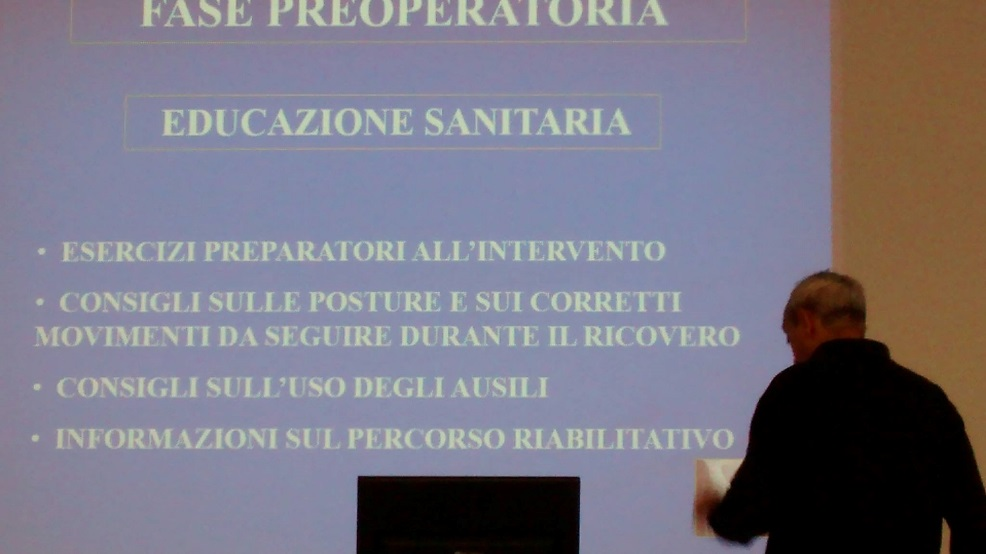
\includegraphics[width=0.5\textwidth]{032/image1.jpeg}
\end{figure}


Il compito del fisiatra è raccomandare al paziente di \emph{svolgere
attività fisica per arrivare all'intervento chirurgico con un buon tono
muscolare}.

\paragraph{Indicazioni e Controindicazioni per l'Artroprotesi d'Anca}


Sono indicazioni per l'impianto di un'artroprotesi d'anca le artrosi
primarie dell'anca, o le artrosi secondarie ad esempio ad epifisiolisi,
a lussazioni congenite o a coxa plana dell'anca, ma non bisogna
dimenticare anche la necrosi asettica della testa del femore per terapia
cortisonica o per irradiazione, l'artrite reumatoide, gli esiti di
fratture del collo del femore, gli esiti di artrodesi o di lussazioni
traumatiche dell'anca, le osteotomie non riuscite ed i tumori ossei
dell'acetabolo e della porzione prossimale del femore.

Sono invece controindicazioni assolute all'esecuzione dell'artroprotesi
d'anca le artriti settiche dell'anca, le patologie neurologiche
dell'articolazione con insufficienza muscolare e tutte quelle patologie
che conducono ad una rapida distruzione del tessuto osseo.

\paragraph{Tecnica di Esecuzione}


Nell'intervento di artroprotesi, la via di accesso è laterale, col
paziente supino con la coscia verso l'esterno, in modo che il grasso
vada verso il basso. Si procede prima con un'incisione di cute e
sottocute centrata a livello del grande trocantere, poi si incide la
fascia lata longitudinalmente, rivelando il ventaglio gluteo che viene
staccato dalla sua inserzione sul grande trocantere. A questo punto si
espone e si incide la capsula articolare, effettuando quindi una
capsulectomia, sino ad arrivare al collo del femore che viene sezionato
con una sega. Si procede con l'asportazione della testa del femore, e
poi con delle frese si toglie la cartilagine residua finché non viene
esposto l'osso subcondrale. Si può a questo punto procedere con
l'inserzione dell'acetabolo, che viene stabilizzato con delle viti, si
prepara il canale midollare e si inserisce lo stelo, riducendo infine la
testa nel nuovo acetabolo.

\paragraph{Complicanze}


Fondamentalmente, le principali complicanze che determinano il
fallimento delle protesi d'anca sono essenzialmente tre:

\begin{itemize}
\item
  \textbf{Mobilizzazione Asettica}, dovuta alla liberazione di
  microdetriti da usura, che vanno a scatenare una reazione
  infiammatoria all'interfaccia osso-protesi. La diagnosi è
  essenzialmente clinica, con un paziente che riferisce dolore al
  fianco, e viene poi confermata da un Rx che mette in evidenza i segni
  dell'usura, e da una scintigrafia ossea. Il trattamento prevede una
  revisione in un unico tempo; si toglie la vecchia protesi e se ne
  impianta una nuova.
\item
  \textbf{Mobilizzazione Settica}, in cui un'infezione può svilupparsi
  anche a distanza dall'impianto, determinando una mobilizzazione della
  protesi. È più rara, ed il paziente può manifestare segni locali di
  flogosi, arrossamento della ferita, fistolizzazione a livello della
  precedente ferita, con fuoriuscita di pus, aumento degli indici di
  flogosi ed Rx che mette in luce dei segni di mobilizzazione. La
  scintigrafia ossea è normale, e viene associata quella dei leucociti
  marcati; se vi è positività ad entrambe le scintigrafie vuol dire che
  i leucociti vanno ad attaccarsi nella zona di infezione. In questo
  caso il trattamento molto raramente è in un unico tempo, più spesso si
  deve prima togliere la protesi, bonificare il focolaio di infezione,
  effettuare dei lavaggi, mettere uno spaziatore in cemento con
  antibiotici e solo successivamente si può procedere alla rimozione
  dello spaziatore e all'impianto delle nuova protesi.
\item
  \textbf{Fratture Periprotesiche}, come nei soggetti anziani che cadono
  e si rompono il femore attorno alla protesi. In questo caso, se lo
  stelo è mobilizzati lo si deve revisionare, mettendone uno più lungo,
  se invece non è mobilizzato si provvede a fare un'osteosintesi della
  frattura periprotesica.
\end{itemize}

\begin{quote}
Altre complicanze possibili sono poi l'anemizzazione post-operatoria, la
comparsa di ematomi locali, la TVP e la TEP, danni nervosi o vascolari,
le ossificazioni eterotipiche, le cicatrici cheloidee, il dolore cronico
in sede di interventi e le dismetrie degli arti, che possono anche
causare zoppia.
\end{quote}

\subsection{Post-intervento}


Nel post-intervento il trattamento è sovrapponibile a quello successivo
a protesi di ginocchio, ma a differenza di questo non abbiamo bisogno
della kinesiterapia passiva.

Normalmente è sufficiente che il paziente inizi a \emph{muovere} prima
\emph{l'arto} controlaterale e poi l'arto operato lavorando su:

\begin{enumerate}
\def\labelenumi{\arabic{enumi}.}
\item
  \begin{quote}
  caviglia, con movimenti di dorso-flessione
  \end{quote}
\item
  \begin{quote}
  ginocchio, con movimenti di flesso-estensione.
  \end{quote}
\end{enumerate}

Il paziente, stando sul lettino e facendo questi movimenti, lavora in
\textbf{catena cinetica chiusa} e quindi usa tutte e tre le
articolazioni dell'arto inferiore e l'anca lavora molto di meno ed
indirettamente: infatti si chiede al paziente di flettere ed estendere
il ginocchio, ma, dal momento che è steso sul lettino, questo movimento
comporta anche la flesso-estensione dell'anca. In questo modo il
paziente è concentrato sul ginocchio e non ha la percezione di lavorare
sull'anca.

Successivamente il paziente deve \emph{mettersi seduto} sul lettino. In
questa posizione flette le ginocchia ma allo stesso tempo l'anca deve
adeguarsi all'altezza del lettino e alla posizione del ginocchio.

In alcuni pazienti che hanno subito interventi di riduzione e sintesi
con chiodo gamma non è possibile sfruttare il movimento attivo e quindi
è necessario far lavorare l'anca in passivo con l'aiuto del
fisioterapista.

La valutazione del paziente viene fatta dal fisiatra in modo da
valutare:

\begin{itemize}
\item
  qual è la situazione del soggetto
\item
  quale trattamento eseguire
\item
  se ci sono delle disabilità.
\end{itemize}

Per ogni tipo di intervento chirurgico ci sono delle scale di
valutazione.

Nelle protesi d'anca si utilizza la \textbf{scala WOMAC} che valuta:

\begin{itemize}
\item
  dolore
\item
  funzionalità
\item
  capacità del soggetto di svolgere le attività quotidiane.
\end{itemize}

Sono scale che vengono utilizzare per avere un'indicazione della
condizione del soggetto prima e dopo il trattamento.

Il trattamento riabilitativo è simile a quello del ginocchio:

\begin{enumerate}
\def\labelenumi{\arabic{enumi})}
\item
  posizionamento a letto, esercizi
\item
  mobilizzazione
\item
  cammino.
\end{enumerate}

\subsection{La dimissione}


Per il paziente sottoposto a un intervento programmato che si trova in
condizioni ottimali, il trattamento riabilitativo non andrà fatto nella
struttura pubblica ma andrà fatto a domicilio o ambulatorialmente.

Le cose cambiano nel paziente traumatico o con co-morbilità. Questi
andranno in strutture riabilitative pubbliche.

In generale il \emph{trattamento riabilitativo a domicilio} è riservato
a pazienti:

\begin{itemize}
\item
  \emph{collaboranti}
\item
  \emph{con familiari collaboranti -> care giver}
\item
  \emph{in buone condizioni internistiche}
\item
  \emph{che vivono in appartamenti senza barriere architettoniche}
\item
  \emph{con un servizio riabilitativo territoriale che provvede a
  inviare il fisioterapista a domicilio (questo è il caso della AUSL di
  Parma).}
\end{itemize}

I \emph{pazienti ambulatoriali} invece sono quelli che hanno delle
barriere architettoniche in casa (che rendono difficile il trattamento
riabilitativo) ma hanno le stesse caratteristiche cliniche di quello
domiciliato (cioè è collaborante e si trova in buone condizioni
internistiche). Il trattamento ambulatoriale viene fatto presso la
struttura ospedaliera o sul territorio.

I \emph{pazienti ricoverati} sono quelli con problematiche internistiche
o poco collaboranti o con problematiche familiari.

Per i pazienti che hanno un età superiore ai 65 anni si consiglia un
\emph{\textbf{trattamento intensivo}} ovvero un trattamento
riabilitativo di un'ora al giorno.

Nei pazienti invece di età più giovane si deve procedere con un
\emph{\textbf{trattamento estensivo}}, cioè di più di 3 ore al giorno.

\subsection{Trattamento riabilitativo nelle fasi successive alla dimissione}


Consiste in:

\begin{itemize}
\item
  rinforzo della muscolatura glutea, adduttoria e quadricipitale e anche
  della componente flessoria.
\item
  Recupero completo del R.O.M. (range of motion) di quell'articolazione.
\item
  Inizio del cammino a 4 tempi con bastoni antibrachiali o canadesi per
  1 mese. Successivamente con 1 bastone. Poi abbandono completo.
\end{itemize}

Ultimamente si assiste ad un trend in aumento di giovani sottoposti ad
interventi chirurgici per sindrome da \textbf{conflitto
femoro-acetabolare}, caratterizzata da un attrito nell'articolazione
coxo-acetabolare, e durante l'intervento vengono rimossi osteofiti.

Questi pazienti da un punto di vista riabilitativo non sono in grado di
recuperare bene il R.O.M. e sono dei candidati per un successivo
intervento di protesi d'anca.

\section{Deep oscillation}


\emph{Avviso: si tratta di un argomento nuovo che il Prof tratterà
l'anno prossimo. Ha deciso di parlarcene brevemente e di fare un
accenno. Io ho cercato su Internet qualche ``approfondimento''.}

Si tratta di un apparecchio costituito da un carrello con un portatile.

\emph{Si basa su un campo a impulsi elettrostatici che vengono prodotti
sulla regione corporea da trattare e la cui frequenza può variare tra 5
e 250 Hz, a seconda dell'indicazione terapeutica scelta.}

Il fisiatra indossa dei guanti e in uno di questi è presente un
elettrodo. L'altro elettrodo viene tenuto in mano dal paziente.

Sulla cute viene applicato del talco perché è un conduttore elettrico.

\emph{Con il movimento dell'applicatore manuale sulla pelle del paziente
si ottiene un effetto di vibrazione ed oscillazione nei tessuti
sottostanti con un'efficacia fino in profondità. Il trattamento
contribuisce a una rigenerazione più rapida dei tessuti in seguito a
traumi e lesioni dovute al sovrallenamento e interventi chirurgici.}

\emph{Le oscillazioni agiscono in maniera assolutamente non invasiva e
fino in profondità su tutte le parti del di tessuto trattate (cute,
epidermide, tessuto adiposo sottocutaneo, muscoli, sangue e
vasi-linfatici).}

\emph{Gli effetti fisiologici sono documentati clinicamente su:
riduzione del dolore, azione antiinfiammatoria, edemi, azione
cicatrizzante, azione antifibrotica, miglioramento dell'atroficità.}

Le \emph{indicazioni} sono le stesse della diatermia.

\emph{Controindicazione}: pazienti con pacemaker, donne gravide o con
tumori.

\begin{figure}[!ht]
\centering
	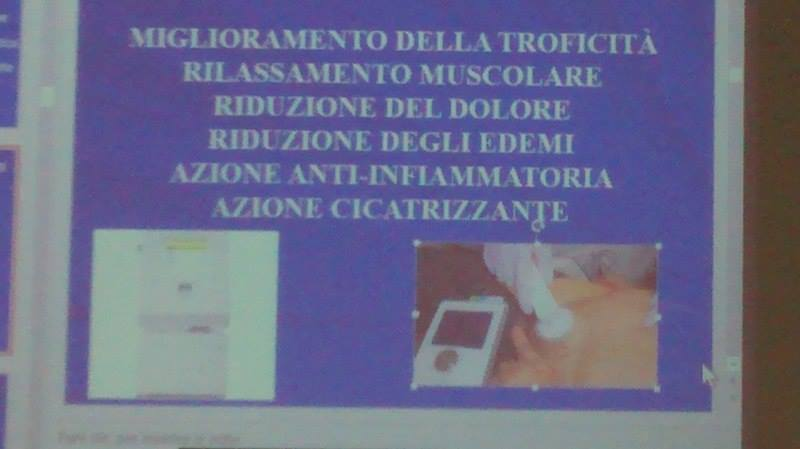
\includegraphics[width=0.5\textwidth]{032/image2.jpeg}
\end{figure}
